\section{Introduction}

With the popularity of the Intenet, there are huge amount of text in
the web, and their size is still growing quickly. In order to use
them, it is of utmost importance to develop automatic nature language
processing (NLP) systems to handle the big data. 

%A typical NLP system would first employ syntactic processing and then
%employ semantic processing.  Syntactic processing is often task
%independent. It aims to convert the raw text into some machine
%friendly structures. The pipeline often includes tokenization, POS
%tagging, parsing, name entity recognition and coreference. Semantic
%processing is often task dependent. It tries to exploit useful
%information from the text for an end  task. 

It has been wildly accepted that statistical machine learning
approaches are very effective for most NLP problems, such as
parsing~\cite{klein2003accurate}, information
extractions~\cite{banko2007open}, question
answering~\cite{kwok2001scaling} and so on. However, there is a
significant limitation of all the statistical approaches: they need a
lot of training data to learn models. Training data are labeled by
human annotators. In most cases, annotators manually predict the
desired outputs for the inputs. The algorithms then learn from the
training data the statistics and models, which are used to
automatically predict the output of the unlabeled data.   

Generally, dataset labeling for machine learning problems (often
classification) is time consuming and tedious. To make matters worse,
it is even harder for annotators to label NLP problems than to label
standard classification problems.

For a standard classification
problem, human annotators are given a set of labels and a list of
objects. Their jobs are to choose a label for each object. Since
objects are usually independent of each other, local information is
enough for label prediction. Besides, labeling errors, if any, would not
affect the rest of the dataset. Therefore, the user interface for the
annotations could be very simple: plain text or Excel tables are often
enough in many cases. 


But for NLP annotations, the outputs are often structured predictions.
That is, each prediction depends on some other prediction. For
example, Figure~\ref{fig:example_parse_tree} shows how a parsing
algorithm converts a sentence into a tree. It is hard for annotators
to decide the position of a single word in the tree before drawing the
whole tree. Besides, a large group of NLP problems are related to
clustering, such as coreference resolution~\cite{lee2011stanford},
which clusters two or more expressions in a text refer to the same
person or thing. Unlike classification, annotates must acquire some
global information before correctly labeling the clusters. Suppose
there are ``Jeffery Heer", ``Jeff Bilmes", ``Jeff", ``the professor"
in a text. To decide whether which ``Jeff" and which ``professor",
annotator must read the context to know who they are. Transitivity
also makes the clustering annotation very tricky. For example, after
merging some pairs of points, the annotator has created two clusters
$\{$``Jeff, Jeff Bilmes''$\}$ and $\{$``Jeffery Heer, Professor
Heer''$\}$. He then accidentally merges ``Jeff" and ``Jeffery Heer".
It would immediately result in a very large and incorrect cluster.


\begin{figure}
\centering
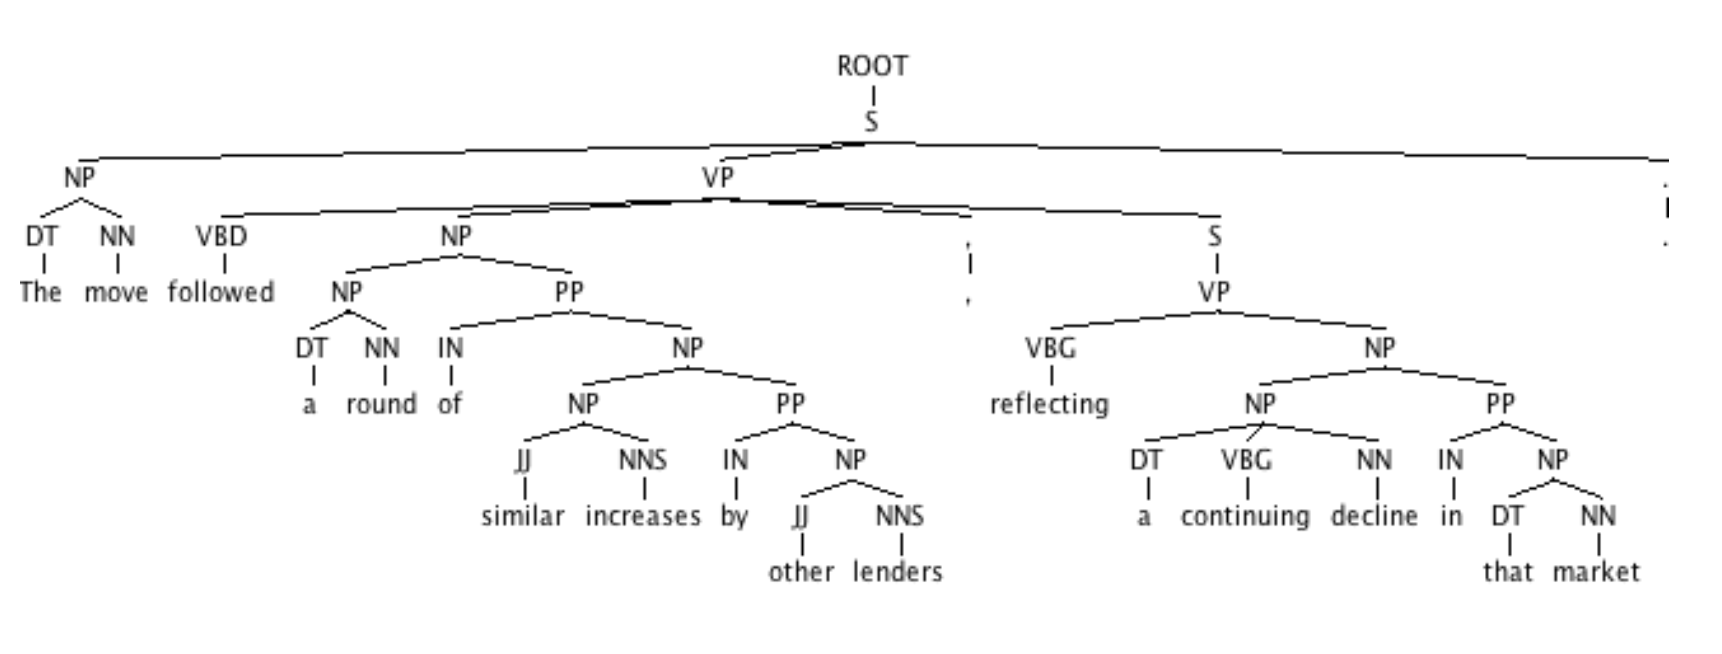
\includegraphics[width=3.1in]{figs/parsetree.png}
\caption{An example parse tree.}
\label{fig:example_parse_tree}
\end{figure}


The challenges listed above make the labeling process uncomfortable
for normal annotators. Firstly, annotators must spend a lot of time to
  understand the global structure of the data before labeling
  anything. Secondly, annotators would often revisit and edit their
  labels. In the above example, the annotator notices that ``Jeff
  Bilmes" and ``Jeffery Heer" are in the same cluster, then he has to
  go back and fix that error. Such trial and errors could cause
  conflicts and incomplete annotations. In fact, even trained
  linguistic must spend a lot of time to label NLP datasets. A famous
  example is that it costs 8 years to create the Penn Tree Bank, a
  labeled dataset of parsed trees. 

Nowadays, there are many worker at crowdsourcing platforms like
Mechanical Turks\footnote{~\url{https://www.mturk.com/mturk/welcome}}
and Odesk. They provide us opportunities to quickly collect a large
amount of training data. But most workers are normal people, having
little knowledge about linguistic, and having no reason to be patient
enough. If the problem is to hard, they would switch to other easier
and profitable jobs. So it is impractical to ask them to label over
plain text files or Excel tables for NLP annotations.  
